\documentclass[12pt,letterpaper]{article}
\usepackage{graphicx,textcomp}
\usepackage{natbib}
\usepackage{setspace}
\usepackage{fullpage}
\usepackage{color}
\usepackage[reqno]{amsmath}
\usepackage{amsthm}
\usepackage{fancyvrb}
\usepackage{amssymb,enumerate}
\usepackage[all]{xy}
\usepackage{endnotes}
\usepackage{lscape}
\newtheorem{com}{Comment}
\usepackage{float}
\usepackage{hyperref}
\newtheorem{lem} {Lemma}
\newtheorem{prop}{Proposition}
\newtheorem{thm}{Theorem}
\newtheorem{defn}{Definition}
\newtheorem{cor}{Corollary}
\newtheorem{obs}{Observation}
\usepackage[compact]{titlesec}
\usepackage{dcolumn}
\usepackage{tikz}
\usetikzlibrary{arrows}
\usepackage{multirow}
\usepackage{xcolor}
\newcolumntype{.}{D{.}{.}{-1}}
\newcolumntype{d}[1]{D{.}{.}{#1}}
\definecolor{light-gray}{gray}{0.65}
\usepackage{url}
\usepackage{listings}
\usepackage{color}

\definecolor{codegreen}{rgb}{0,0.6,0}
\definecolor{codegray}{rgb}{0.5,0.5,0.5}
\definecolor{codepurple}{rgb}{0.58,0,0.82}
\definecolor{backcolour}{rgb}{0.95,0.95,0.92}

\lstdefinestyle{mystyle}{
	backgroundcolor=\color{backcolour},   
	commentstyle=\color{codegreen},
	keywordstyle=\color{magenta},
	numberstyle=\tiny\color{codegray},
	stringstyle=\color{codepurple},
	basicstyle=\footnotesize,
	breakatwhitespace=false,         
	breaklines=true,                 
	captionpos=b,                    
	keepspaces=true,                 
	numbers=left,                    
	numbersep=5pt,                  
	showspaces=false,                
	showstringspaces=false,
	showtabs=false,                  
	tabsize=2
}
\lstset{style=mystyle}
\newcommand{\Sref}[1]{Section~\ref{#1}}
\newtheorem{hyp}{Hypothesis}

\title{Problem Set 3}
\date{Due: November 19, 2022}
\author{Applied Stats/Quant Methods 1 \\ \vspace{\baselineskip}
	 \textbf{Maiia Skrypnyk 23371609}}


\begin{document}
	\maketitle
	\section*{Instructions}
	\begin{itemize}
		\item Please show your work! You may lose points by simply writing in the answer. If the problem requires you to execute commands in \texttt{R}, please include the code you used to get your answers. Please also include the \texttt{.R} file that contains your code. If you are not sure if work needs to be shown for a particular problem, please ask.
	\item Your homework should be submitted electronically on GitHub.
	\item This problem set is due before 23:59 on Sunday November 19, 2023. No late assignments will be accepted.

	\end{itemize}

		\vspace{.25cm}
	
\noindent In this problem set, you will run several regressions and create an add variable plot (see the lecture slides) in \texttt{R} using the \texttt{incumbents\_subset.csv} dataset. Include all of your code.

	\vspace{.5cm}
\section*{Question 1}
\vspace{.25cm}
\noindent We are interested in knowing how the difference in campaign spending between incumbent and challenger affects the incumbent's vote share. 
\begin{enumerate}
		\item Run a regression where the outcome variable is \texttt{voteshare} and the explanatory variable is \texttt{difflog}.	
		
		\lstinputlisting[language=R, firstline=39, lastline=39]{PS03MS.R} 
		
Exploring the model's summary and using 'stargazer' function to format results: 

	\lstinputlisting[language=R, firstline=41, lastline=42]{PS03MS.R} 
	
\begin{table}[!htbp] \centering   \caption{Model 1: Campaign Spending Difference vs. Incumbent Vote Share} \label{} \begin{tabular}{@{\extracolsep{5pt}}lc} \\[-1.8ex]\hline \hline \\[-1.8ex]  & \multicolumn{1}{c}{\textit{Dependent variable:}} \\ \cline{2-2} \\[-1.8ex] & voteshare \\ \hline \\[-1.8ex]  difflog & 0.042$^{***}$ \\   & (0.001) \\   & \\  Constant & 0.579$^{***}$ \\   & (0.002) \\   & \\ \hline \\[-1.8ex] Observations & 3,193 \\ R$^{2}$ & 0.367 \\ Adjusted R$^{2}$ & 0.367 \\ Residual Std. Error & 0.079 (df = 3191) \\ F Statistic & 1,852.791$^{***}$ (df = 1; 3191) \\ \hline \hline \\[-1.8ex] \textit{Note:}  & \multicolumn{1}{r}{$^{*}$p$<$0.1; $^{**}$p$<$0.05; $^{***}$p$<$0.01} \\ \end{tabular} \end{table} > 

On average, a one unit increase in \textit{Difflog} (campaign spending difference between incumbent and challenger) is associated with 0.042 unit increase in \textit{Voteshare} (incumbent's vote share). If \(H_0: \hat{\beta}_1 = 0\), given that our p-value is less than 0.01*, we can reject the null hypothesis that there is no association between \textit{Difflog} and \textit{Voteshare}. 

*The estimated coefficient is statistically differentiable from 0 at the \alpha \ \text{level} = 0.05.

		\item Make a scatterplot of the two variables and add the regression line. 
		
			\lstinputlisting[language=R, firstline=44, lastline=53]{PS03MS.R} 
			
		\begin{figure}[H]
			\centering
			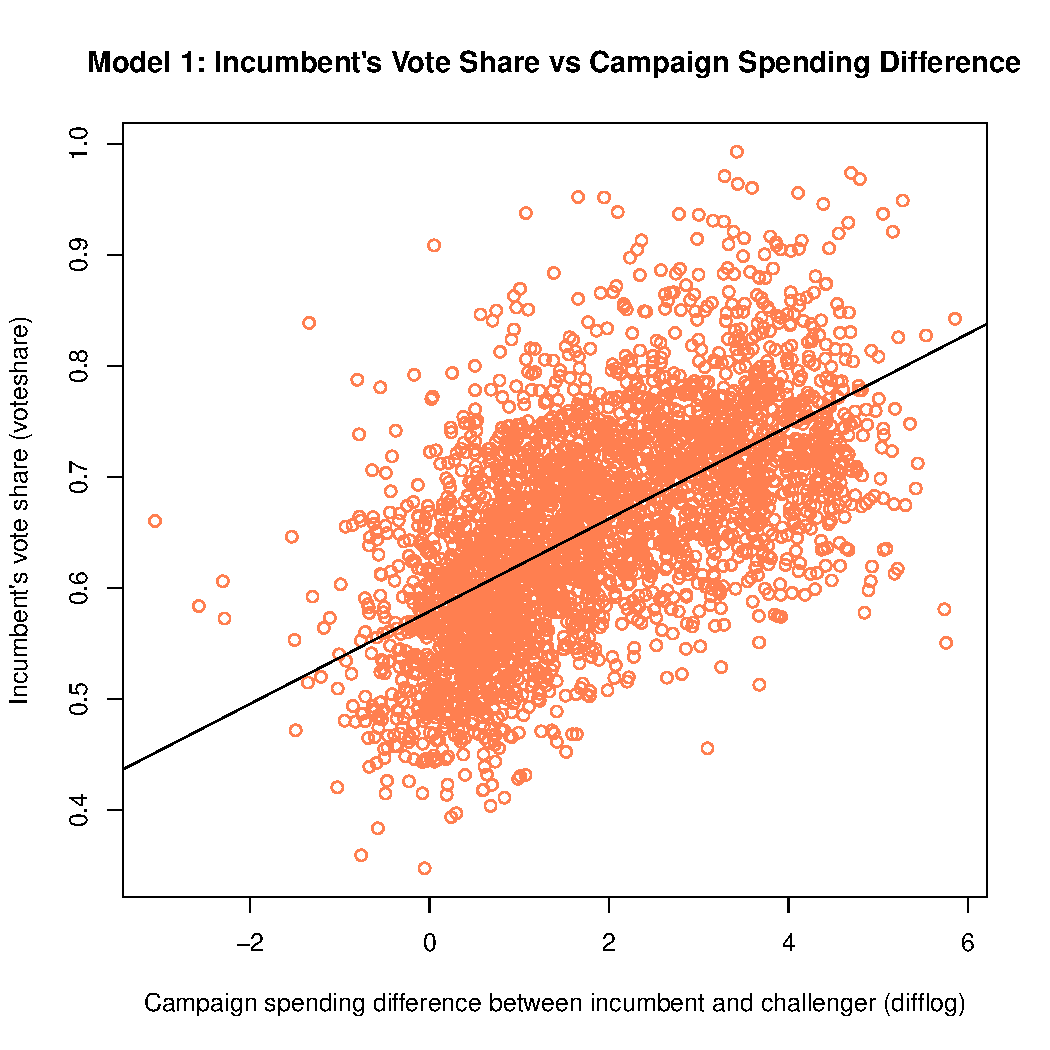
\includegraphics[width=0.6\textwidth]{01.PS03_Skrypnyk_Plot1.pdf}
			\caption{Scatterplot for Model 1}
			\label{fig:Plot1}
		\end{figure}

By analysing the scatterplot, we can see that there is a positive association between the variables (although with outliers).
		
		\item Save the residuals of the model in a separate object.	
	\lstinputlisting[language=R, firstline=56, lastline=56]{PS03MS.R} 
	
		\item Write the prediction equation.
		
\textit{*Chatterjee and Hadi, 2012, p.41}
\begin{center}
	
	\[
	\hat{y_i} = \hat{\beta}_0 + \hat{\beta}_1 \cdot x_i
	\]
	\[\hat{\textbf{\textit{Voteshare}}}_i  = \hat{\beta}_0 + \hat{\beta}_1 \cdot  \textit{Difflog}_i
	\]
\end{center}

\begin{flushleft}
	
\begin{itemize}
	\item $\hat{\textit{y}}_i = \hat{\textbf{\textit{Voteshare}}}_i$ = predicted value of the response variable (incumbent's vote share)
	\item $\hat{\beta}_0$ = estimated intercept
	\item $\hat{\beta}_1$ = estimated slope coefficient
	\item $x_i$ = \textit{Difflog}\(_i\) = (any chosen) value of the explanatory variable (difference in campaign spending between incumbent and challenger candidates)
\end{itemize}

	
\end{flushleft}
		\[\hat{\textbf{\textit{Voteshare}}}_i  =  0.579 + 0.042 \cdot  \textit{Difflog}_i
	\]

	\end{enumerate}

\section*{Question 2}
\noindent We are interested in knowing how the difference between incumbent and challenger's spending and the vote share of the presidential candidate of the incumbent's party are related.	\vspace{.25cm}
	\begin{enumerate}
		\item Run a regression where the outcome variable is \texttt{presvote} and the explanatory variable is \texttt{difflog}.	
		
		\lstinputlisting[language=R, firstline=61, lastline=61]{PS03MS.R} 
		
		Exploring the model's summary and using 'stargazer' function to format results: 
		
			\lstinputlisting[language=R, firstline=64, lastline=65]{PS03MS.R} 
		\begin{table}[H] \centering   \caption{Model 2: Presidential Candidate (Incumbent Party) Vote Share vs Campaign Spending Difference}   \label{} \begin{tabular}{@{\extracolsep{5pt}}lc} \\[-1.8ex]\hline \hline \\[-1.8ex]  & \multicolumn{1}{c}{\textit{Dependent variable:}} \\ \cline{2-2} \\[-1.8ex] & presvote \\ \hline \\[-1.8ex]  difflog & 0.024$^{***}$ \\   & (0.001) \\   & \\  Constant & 0.508$^{***}$ \\   & (0.003) \\   & \\ \hline \\[-1.8ex] Observations & 3,193 \\ R$^{2}$ & 0.088 \\ Adjusted R$^{2}$ & 0.088 \\ Residual Std. Error & 0.110 (df = 3191) \\ F Statistic & 307.715$^{***}$ (df = 1; 3191) \\ \hline \hline \\[-1.8ex] \textit{Note:}  & \multicolumn{1}{r}{$^{*}$p$<$0.1; $^{**}$p$<$0.05; $^{***}$p$<$0.01} \\ \end{tabular} \end{table} 
 
 On average, a one unit increase in \textit{Difflog} (campaign spending difference between incumbent and challenger) is associated with 0.024 unit increase in \textit{Presvote} (presidential candidate's from the incumbent party vote share). If \(H_0: \hat{\beta}_1 = 0\), given that our p-value is less than 0.01*, we can reject the null hypothesis that there is no association between \textit{Difflog} and \textit{Presvote}. 
 
 *The estimated coefficient is statistically differentiable from 0 at the \alpha \ \text{level} = 0.05. 
 
		\item Make a scatterplot of the two variables and add the regression line.
		
				\lstinputlisting[language=R, firstline=67, lastline=77]{PS03MS.R}  
		
			\begin{figure}[H]
			\centering
			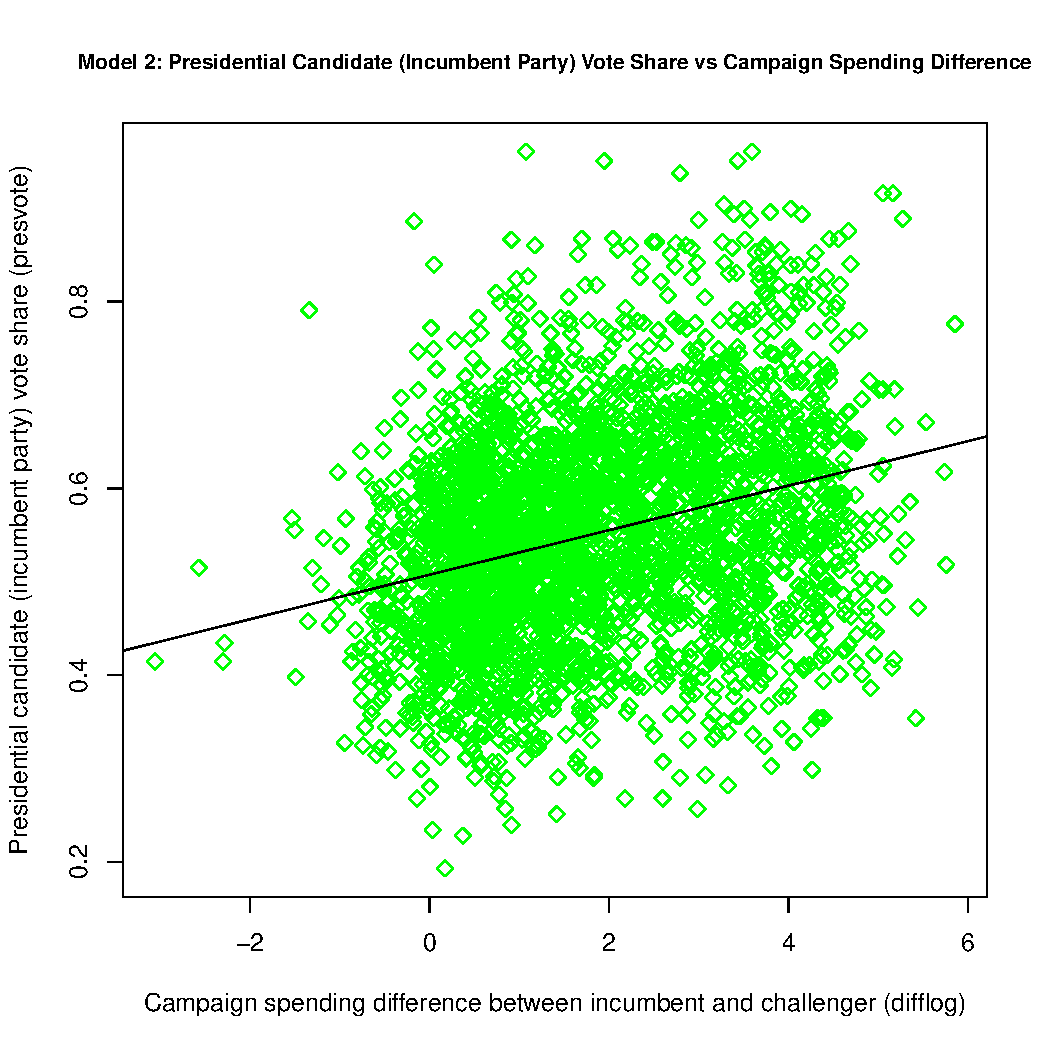
\includegraphics[width=0.6\textwidth]{02.PS03_Skrypnyk_Plot2.pdf}
			\caption{Scatterplot for Model 2}
			\label{fig:Plot2}
		\end{figure}
		
Analysing the scatterplot, we can see (similarly to the previous one) that there is a positive association between the variables (although with outliers). 

		\item Save the residuals of the model in a separate object.	
		
			\lstinputlisting[language=R, firstline=80, lastline=80]{PS03MS.R}  
			
		\item Write the prediction equation.
	\begin{center}
		
		\[
		\hat{y_i} = \hat{\beta}_0 + \hat{\beta}_1 \cdot x_i
		\]
		\[\hat{\textbf{\textit{Presvote}}}_i  = \hat{\beta}_0 + \hat{\beta}_1 \cdot  \textit{Difflog}_i
		\]
	\end{center}
		
		\begin{flushleft}
			
		\begin{itemize}
			\item $\hat{\textit{y}}_i = \hat{\textbf{\textit{Presvote}}}_i$ = predicted value of the response variable (vote share of the presidential candidate from the incumbent party)
			\item $\hat{\beta}_0$ = estimated intercept
			\item $\hat{\beta}_1$ = estimated slope coefficient
			\item $x_i$  =\textit{Difflog}\(_i\) = (any chosen) value of the explanatory variable (difference in campaign spending between incumbent and challenger candidates)
		\end{itemize}
		
			
		\end{flushleft}
		\[\hat{\textbf{\textit{Presvote}}}_i  =  0.508 + 0.024\cdot  \textit{Difflog}_i
		\]
		
	\end{enumerate}
	
\section*{Question 3}

\noindent We are interested in knowing how the vote share of the presidential candidate of the incumbent's party is associated with the incumbent's electoral success.
	\vspace{.25cm}
	\begin{enumerate}
		\item Run a regression where the outcome variable is \texttt{voteshare} and the explanatory variable is \texttt{presvote}.
		
			\lstinputlisting[language=R, firstline=85, lastline=85]{PS03MS.R} 
		
		Exploring the model's summary and using 'stargazer' function to format results: 
		
		\lstinputlisting[language=R, firstline=88, lastline=89]{PS03MS.R} 
		
		\begin{table}[H] \centering   \caption{Model 3: Incumbent's Vote Share vs. Presidential Candidate (Incumbent Party) Vote Share}   \label{} \begin{tabular}{@{\extracolsep{5pt}}lc} \\[-1.8ex]\hline \hline \\[-1.8ex]  & \multicolumn{1}{c}{\textit{Dependent variable:}} \\ \cline{2-2} \\[-1.8ex] & voteshare \\ \hline \\[-1.8ex]  presvote & 0.388$^{***}$ \\   & (0.013) \\   & \\  Constant & 0.441$^{***}$ \\   & (0.008) \\   & \\ \hline \\[-1.8ex] Observations & 3,193 \\ R$^{2}$ & 0.206 \\ Adjusted R$^{2}$ & 0.206 \\ Residual Std. Error & 0.088 (df = 3191) \\ F Statistic & 826.950$^{***}$ (df = 1; 3191) \\ \hline \hline \\[-1.8ex] \textit{Note:}  & \multicolumn{1}{r}{$^{*}$p$<$0.1; $^{**}$p$<$0.05; $^{***}$p$<$0.01} \\ \end{tabular} \end{table} 
		
 On average, a one unit increase in \textit{Presvote} (presidential candidate's from the incumbent party vote share) is associated with 0.388 unit increase in \textit{Voteshare} (incumbent's vote share). It should be noted that this is large value for a slope coefficient, especially compared to the previous two models. If \(H_0: \hat{\beta}_1 = 0\), given that our p-value is less than 0.01*, we can reject the null hypothesis that there is no association between \textit{Presvote} and \textit{Voteshare}. 
 
 *The estimated coefficient is statistically differentiable from 0 at the \alpha \ \text{level} = 0.05.
		
		\item Make a scatterplot of the two variables and add the regression line. 

	\lstinputlisting[language=R, firstline=91, lastline=102]{PS03MS.R} 

				\begin{figure}[H]
				\centering
				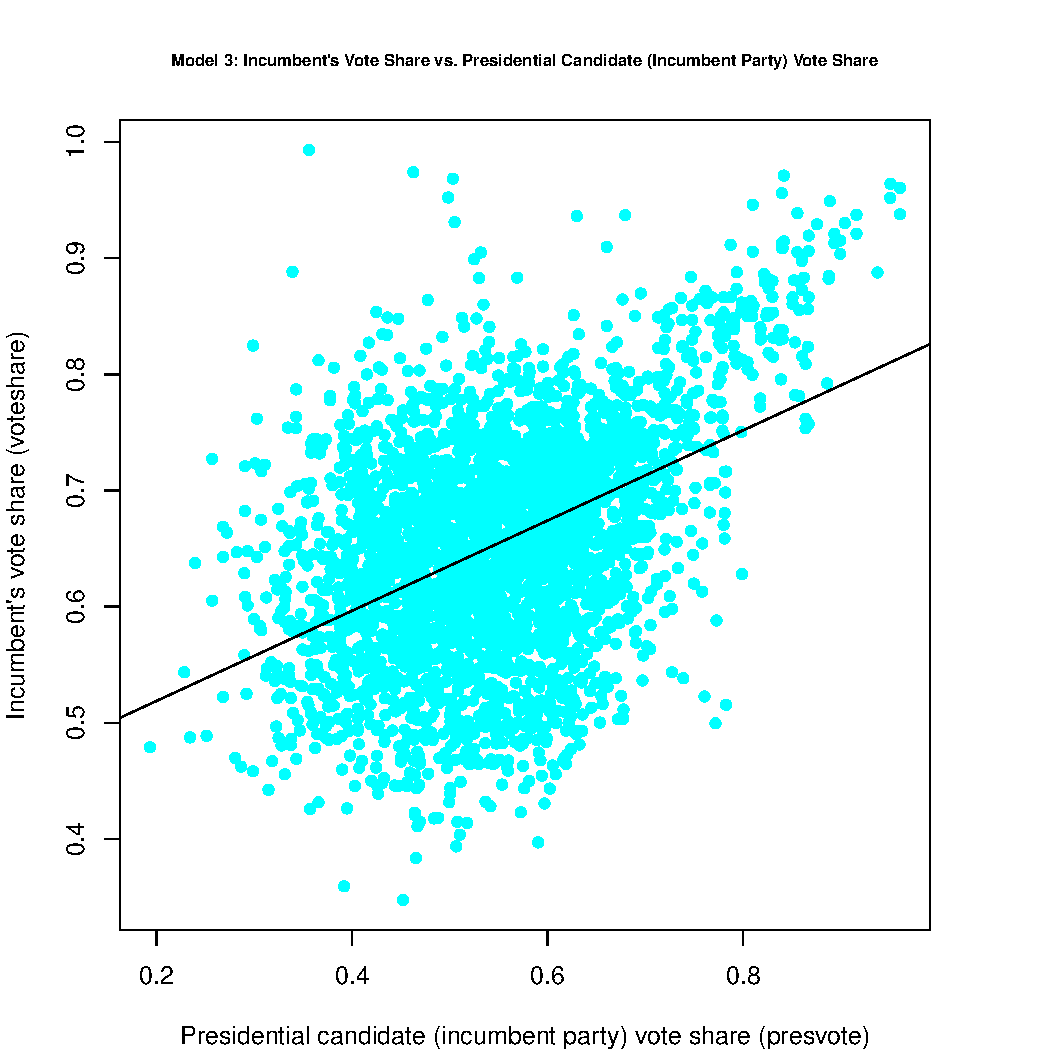
\includegraphics[width=0.6\textwidth]{03.PS03_Skrypnyk_Plot3.pdf}
				\caption{Scatterplot for Model 3}
				\label{fig:Plot3}
			\end{figure}
			
Analysing the scatterplot, we can see (similarly to the previous ones) that there is a positive association between the variables (although with outliers). 
			
		\item Write the prediction equation.
	

	\begin{center}
	
	\[
	\hat{y_i} = \hat{\beta}_0 + \hat{\beta}_1 \cdot x_i
	\]
	\[\hat{\textbf{\textit{Voteshare}}}_i  = \hat{\beta}_0 + \hat{\beta}_1 \cdot  \textit{Presvote}_i
	\]
\end{center}

\begin{flushleft}
	
\begin{itemize}
	\item $\hat{\textit{y}}_i = \hat{\textbf{\textit{Voteshare}}}_i$ = predicted value of the response variable (estimated incumbent's vote share)
	\item $\hat{\beta}_0$ = estimated intercept
	\item $\hat{\beta}_1$ = estimated slope coefficient
	\item $x_i = \textit{Presvote}_i$ = (any chosen) value of the explanatory variable (vote share of the presidential candidate from the incumbent party)
\end{itemize}

\end{flushleft}
\[\hat{\textbf{\textit{Voteshare}}}_i  =  0.441 + 0.388\cdot  \textit{Presvote}_i
\]

	\end{enumerate}

\section*{Question 4}
\noindent The residuals from part (a) tell us how much of the variation in \texttt{voteshare} is $not$ explained by the difference in spending between incumbent and challenger. The residuals in part (b) tell us how much of the variation in \texttt{presvote} is $not$ explained by the difference in spending between incumbent and challenger in the district.
	\begin{enumerate}
		\item Run a regression where the outcome variable is the residuals from Question 1 and the explanatory variable is the residuals from Question 2.	
		
			\lstinputlisting[language=R, firstline=107, lastline=107]{PS03MS.R} 
			
				Exploring the model's summary and using 'stargazer' function to format results: 
			
			\lstinputlisting[language=R, firstline=110, lastline=111]{PS03MS.R}
			
\begin{table}[H] \centering   \caption{Model 4: Model 1 Residuals vs. Model 2 Residuals}   \label{} \begin{tabular}{@{\extracolsep{5pt}}lc} \\[-1.8ex]\hline \hline \\[-1.8ex]  & \multicolumn{1}{c}{\textit{Dependent variable:}} \\ \cline{2-2} \\[-1.8ex] & m1res \\ \hline \\[-1.8ex]  m2res & 0.257$^{***}$ \\   & (0.012) \\   & \\  Constant & $-$0.000 \\   & (0.001) \\   & \\ \hline \\[-1.8ex] Observations & 3,193 \\ R$^{2}$ & 0.130 \\ Adjusted R$^{2}$ & 0.130 \\ Residual Std. Error & 0.073 (df = 3191) \\ F Statistic & 476.975$^{***}$ (df = 1; 3191) \\ \hline \hline \\[-1.8ex] \textit{Note:}  & \multicolumn{1}{r}{$^{*}$p$<$0.1; $^{**}$p$<$0.05; $^{***}$p$<$0.01} \\ \end{tabular} \end{table} 

On average, a one unit increase in \textit{Model 2 Residuals} is associated with 0.257 unit increase in \textit{Model 1 Residuals}. It should be noted that this is also a large value for a slope coefficient. If \(H_0: \hat{\beta}_1 = 0\), given that our p-value is less than 0.01*), we can reject the null hypothesis that there is no association between \textit{Model 1 Residuals} and \textit{Model 2 Residuals}. 

*The estimated coefficient is statistically differentiable from 0 at the \alpha \ \text{level} = 0.05.

		\item Make a scatterplot of the two residuals and add the regression line. 

			\lstinputlisting[language=R, firstline=112, lastline=122]{PS03MS.R} 
		
			\begin{figure}[H]
			\centering
			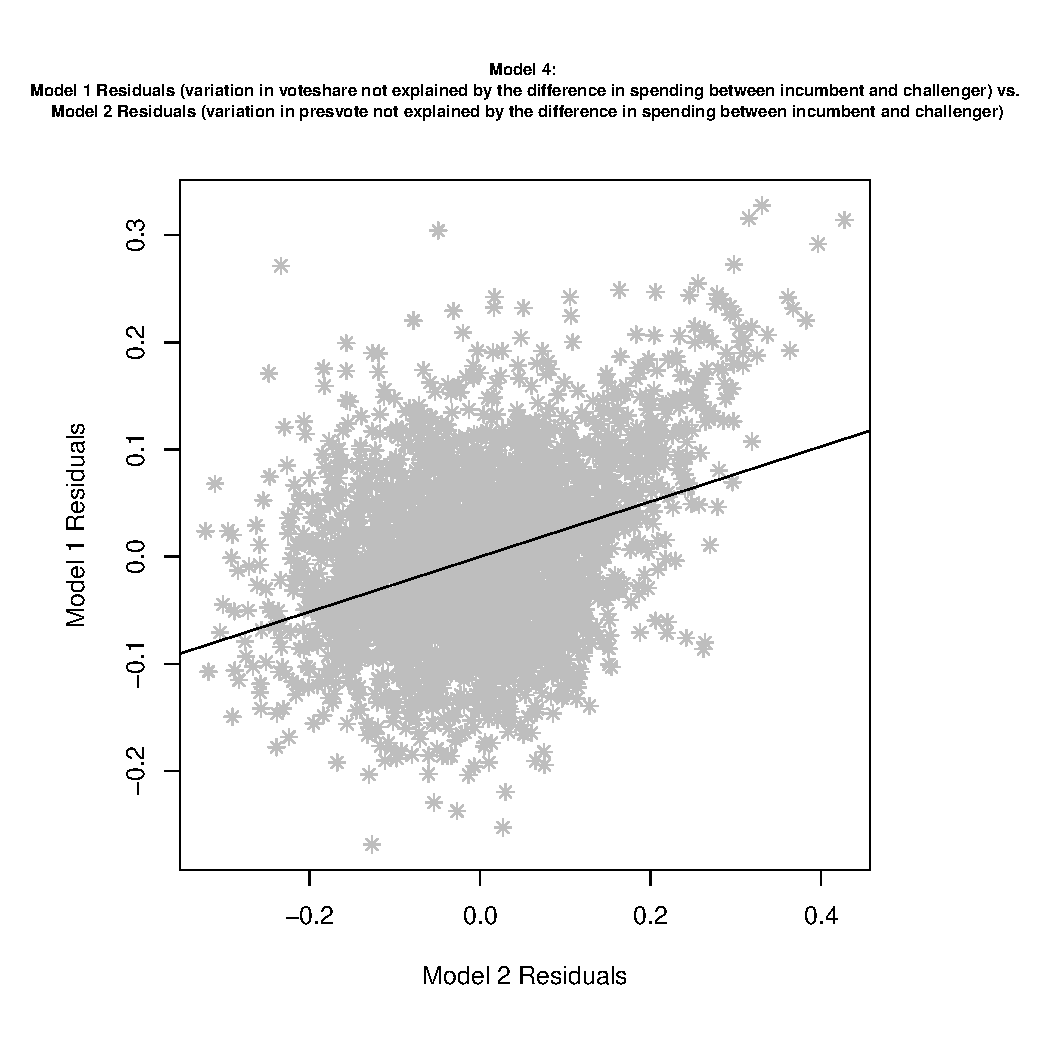
\includegraphics[width=0.6\textwidth]{04.PS03_Skrypnyk_Plot4.pdf}
			\caption{Scatterplot for Model 4}
			\label{fig:Plot4}
		\end{figure}
		
Analysing the scatterplot, we can see (similarly to the previous ones) that there is a positive association between the variables (although with outliers).  

\newpage

		\item Write the prediction equation.
		
	\begin{center}
	
	\[
	\hat{y_i} = \hat{\beta}_0 + \hat{\beta}_1 \cdot x_i
	\]
	\[\hat{\textbf{\textit{m1res}}}_i  = \hat{\beta}_0 + \hat{\beta}_1 \cdot  \textit{m2res}_i
	\]
\end{center}

\begin{flushleft}
	
	\begin{itemize}
		\item $\hat{\textit{y}}_i = \hat{\textbf{\textit{m1res}}}_i$ = predicted value of the response variable -- Model 1 Residuals (tell us how much of the variation in \texttt{voteshare} is $not$ explained by the difference in spending between incumbent and challenger)
		\item $\hat{\beta}_0$ = estimated intercept
		\item $\hat{\beta}_1$ = estimated slope coefficient
		\item $x_i = \textit{m2res}_i$ = (any chosen) value of the explanatory variable -- Model 2 Residuals (tell us how much of the variation in \texttt{presvote} is $not$ explained by the difference in spending between incumbent and challenger in the district) 
	\end{itemize}
	
\end{flushleft}
\[\hat{\textbf{\textit{m1res}}}_i  =  0.257\cdot  \textit{m2res}_i
\]

		\end{enumerate}

\section*{Question 5}
\noindent What if the incumbent's vote share is affected by both the president's popularity and the difference in spending between incumbent and challenger? 

	\begin{enumerate}
		\item Run a regression where the outcome variable is the incumbent's \texttt{voteshare} and the explanatory variables are \texttt{difflog} and \texttt{presvote}.	
		
			\lstinputlisting[language=R, firstline=129, lastline=129]{PS03MS.R} 
		
		Exploring the model's summary and using 'stargazer' function to format results: 
		
		\lstinputlisting[language=R, firstline=132, lastline=133]{PS03MS.R}

\begin{table}[H] \centering   \caption{Model 5: Incumbent's Vote Share vs. Campaign Spending Difference + Presidential Candidate (Incumbent Party) Vote Share}   \label{} \begin{tabular}{@{\extracolsep{5pt}}lc} \\[-1.8ex]\hline \hline \\[-1.8ex]  & \multicolumn{1}{c}{\textit{Dependent variable:}} \\ \cline{2-2} \\[-1.8ex] & voteshare \\ \hline \\[-1.8ex]  difflog & 0.036$^{***}$ \\   & (0.001) \\   & \\  presvote & 0.257$^{***}$ \\   & (0.012) \\   & \\  Constant & 0.449$^{***}$ \\   & (0.006) \\   & \\ \hline \\[-1.8ex] Observations & 3,193 \\ R$^{2}$ & 0.450 \\ Adjusted R$^{2}$ & 0.449 \\ Residual Std. Error & 0.073 (df = 3190) \\ F Statistic & 1,302.947$^{***}$ (df = 2; 3190) \\ \hline \hline \\[-1.8ex] \textit{Note:}  & \multicolumn{1}{r}{$^{*}$p$<$0.1; $^{**}$p$<$0.05; $^{***}$p$<$0.01} \\ \end{tabular} \end{table} 

\begin{itemize}
	\item Holding \textit{Presvote }constant, a one unit increase in \textit{Difflog } (campaign spending difference between incumbent and challenger) is, on average, associated with a 0.036 unit increase in \textit{Voteshare } (the incumbent's vote share). If \(H_0: \hat{\beta}_1 = 0\), given that our p-value is less than 0.01*, we can reject the null hypothesis that there is no association between \textit{Difflog} and \textit{Voteshare} (controlling for other variables).
	\item Holding \textit{Difflog} constant, a one unit increase in \textit{Presvote} (vote share of the presidential candidate from the incumbent party) is, on average, associated with a 0.0257 unit increase in \textit{Voteshare } (the incumbent's vote share). If \(H_0: \hat{\beta}_2 = 0\), given that our p-value is less than 0.01*, we can reject the null hypothesis that there is no association between \textit{Presvote} and \textit{Voteshare} (controlling for other variables).
\end{itemize}

*The estimated coefficient is statistically differentiable from 0 at the \alpha \ \text{level} = 0.05.

		\item Write the prediction equation.
			\begin{center}
			\[
			\hat{y}_i = \hat{\beta}_0 + \hat{\beta}_1 \cdot x_{1i} + \hat{\beta}_2 \cdot x_{2i}
			\]
\[
\hat{\textbf{\textit{Voteshare}}}_i = \hat{\beta}_0 + \hat{\beta}_1 \cdot \textit{\text{Difflog}}_i + \hat{\beta}_2 \cdot \textit{\text{Presvote}}_i
\]

		\end{center}
		
		\begin{flushleft}
			
			\begin{itemize}
				\item $\hat{\textit{y}}_i = \hat{\textbf{\textit{Voteshare}}}_i$ = predicted value of the response variable (incumbent's vote share)
				\item $\hat{\beta}_0$ = estimated intercept
				\item $\hat{\beta}_1$ = estimated slope coefficient for \textit{Difflog}
				\item $x_ 1= \textit{Difflog}_i$ = (any chosen) value of the first explanatory variable (difference in campaign spending between incumbent and challenger candidates)
				\item $\hat{\beta}_2$ = estimated slope coefficient for \textit{Presvote}
				\item $x_ 1= \textit{Presvote}_i$ = (any chosen) value of the second explanatory variable (vote share of the presidential candidate from the incumbent party)
			\end{itemize}
			
		\end{flushleft}
		\[\hat{\textbf{\textit{Voteshare}}}_i  =  0.449 + 0.036\cdot  \textit{Difflog}_i + 0.257\cdot  \textit{Presvote}_i 
		\]
		
		\item What is it in this output that is identical to the output in Question 4? Why do you think this is the case?
	
From the result tables, we can see that a slope coefficient $\hat{\beta}_1$ for \textit{m2res\_i} (Table 4) and $\hat{\beta}_1$ for \textit{Presvote}  over \textit{Voteshare }(\textit{Difflog} controlled for)(Table 5) are identical = 0.257.

In Model 4, our outcome variable is \textit{Model 1 Residuals} that tells us how much of the variation in \textit{Voteshare} is \textbf{not }explained by \textit{Difflog } and our explanatory variable is \textit{Model 2 Residuals} that tells us how much of the variation in \textit{Presvote} is \textbf{not }explained by Difflog. 

Multiple linear regression analysis allows us to estimate the association between an outcome variable and an explanatory variable \textbf{holding all other variables constant. } In Model 5, we run a multivariate regression of \textit{Voteshare} over both \textit{Presvote} and \textit{Difflog}. Therefore, $\hat{\beta}_1$ for \textit{Presvote}  (\textit{Difflog} controlled for) represents the variance for  \textit{Voteshare} explained by \textit{Presvote} and \textbf{not} explained by \textit{Difflog}  -- similarly to Model 4.

We can also see that the Residual Standard Errors of both models = 0.073, so let's also check whether  the residuals of these two models are identical (as they should be):

\lstinputlisting[language=R, firstline=135, lastline=140]{PS03MS.R} 


	\end{enumerate}
\end{document}
